\begin{figure}[htb!]
\centering
\begin{small}
\begin{tabular}{lll}
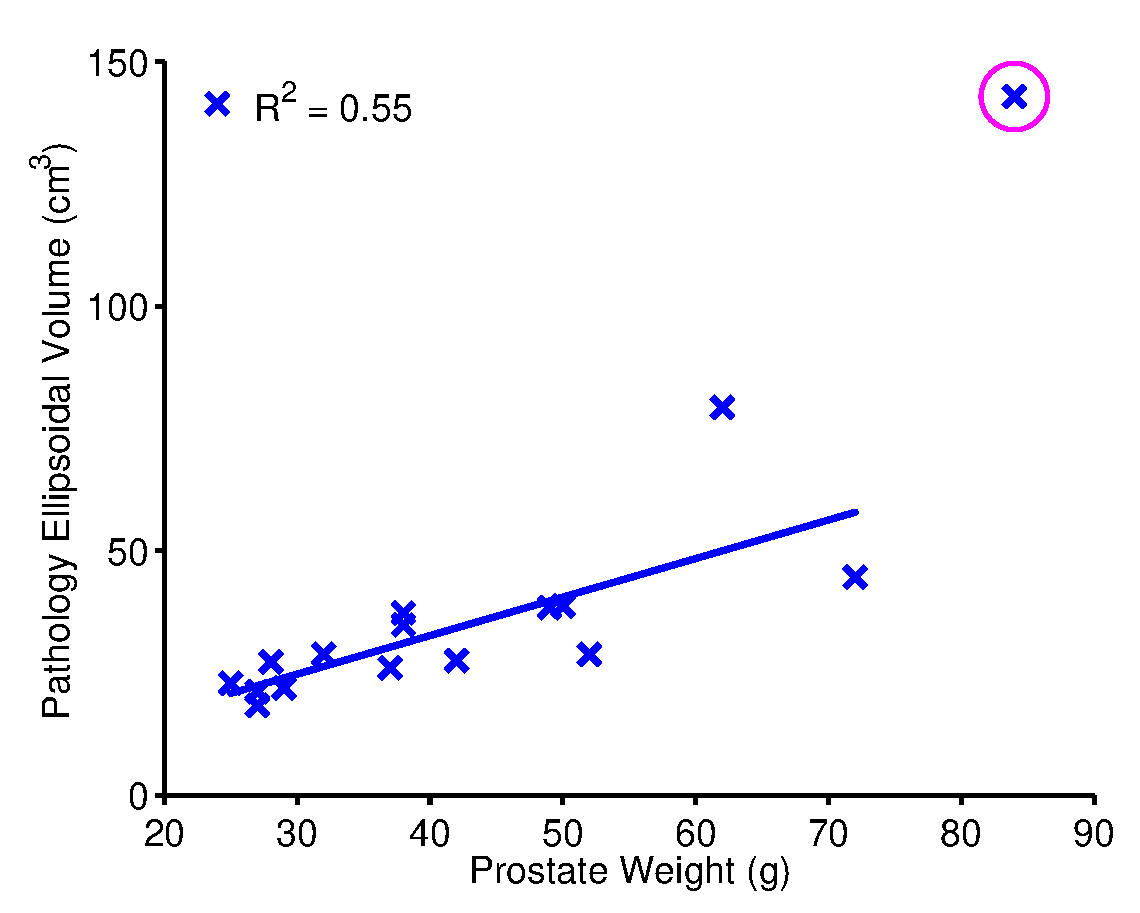
\includegraphics[width=0.3\linewidth]{figs/corr_path_vol_weight_vol} &
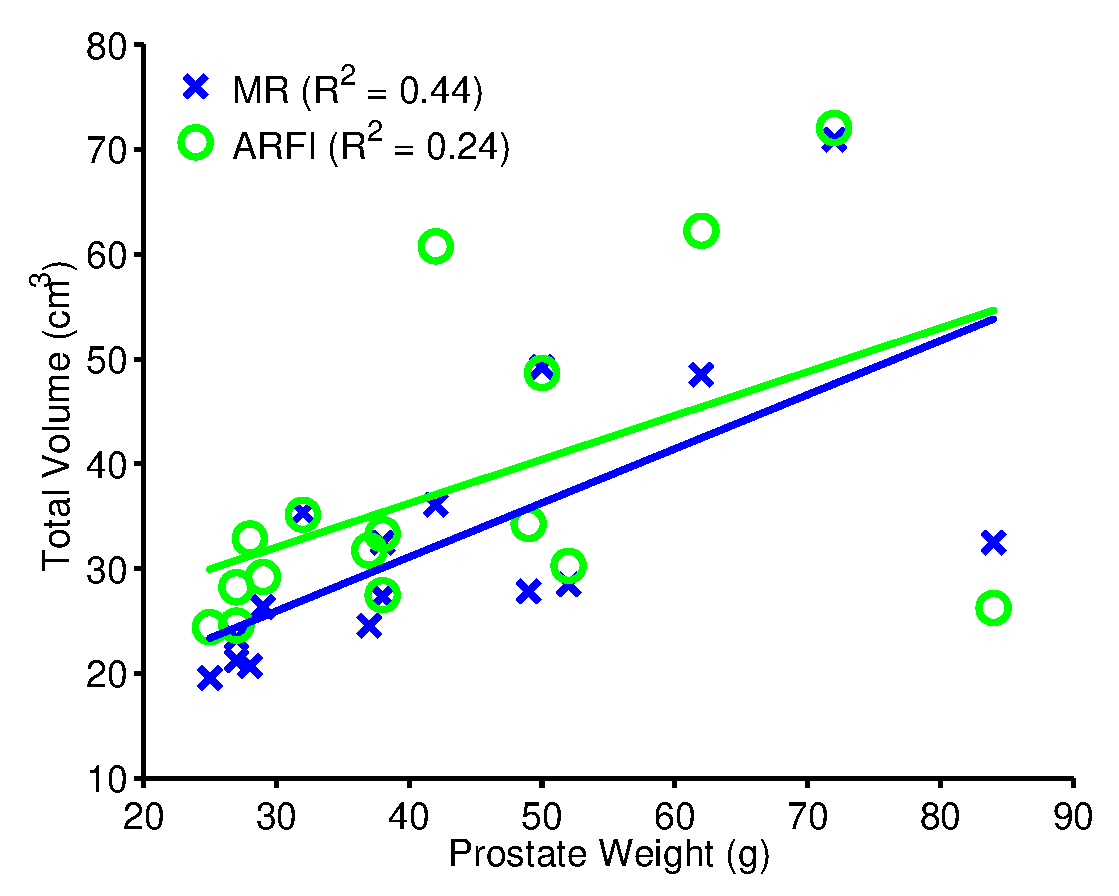
\includegraphics[width=0.3\linewidth]{figs/corr_weight_vol} &
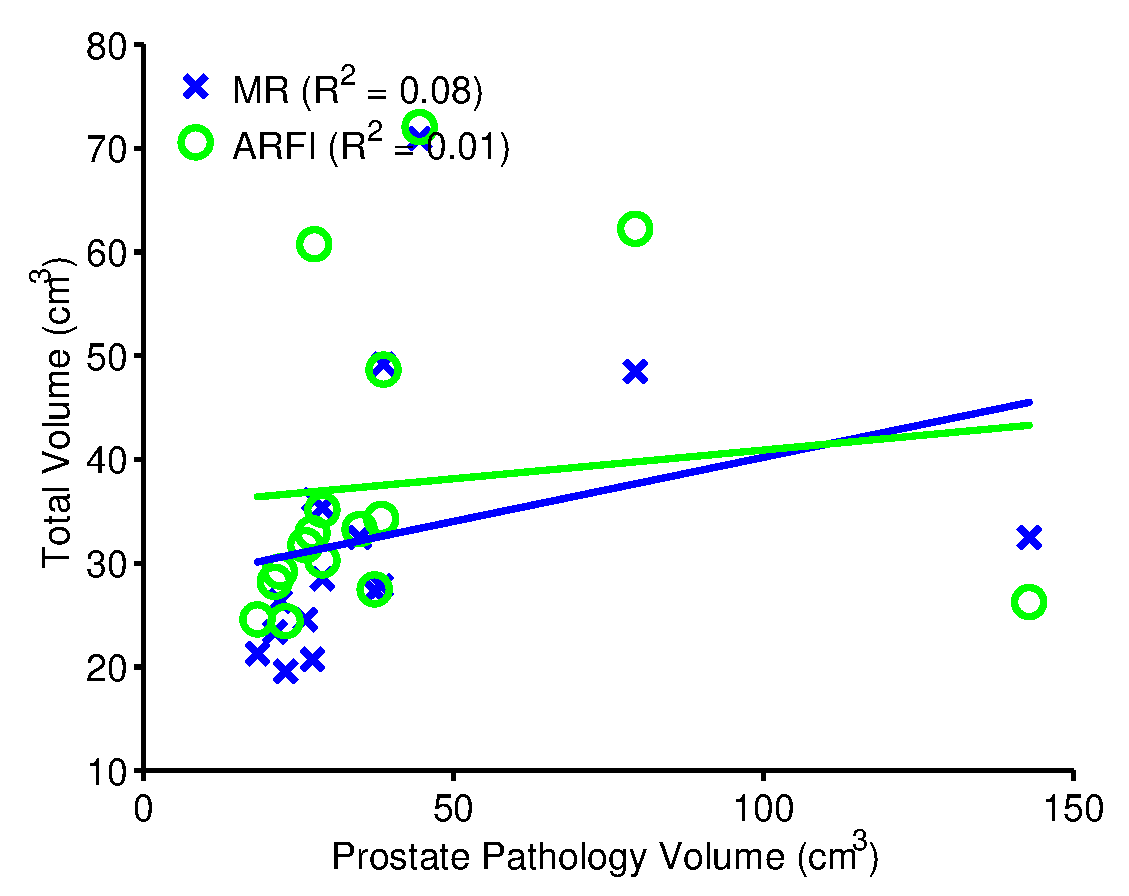
\includegraphics[width=0.3\linewidth]{figs/corr_pathVol_vol} \\
(a) Prostate Weight : Prostate Volume & (b) Image Volume : Prostate Weight & (c) Image Volume : Prostate Volume \\
\end{tabular}
\end{small}
%\begin{tabular}{ll}
%\includegraphics[width=0.3\linewidth]{figs/corr_weight_vol_no4} &
%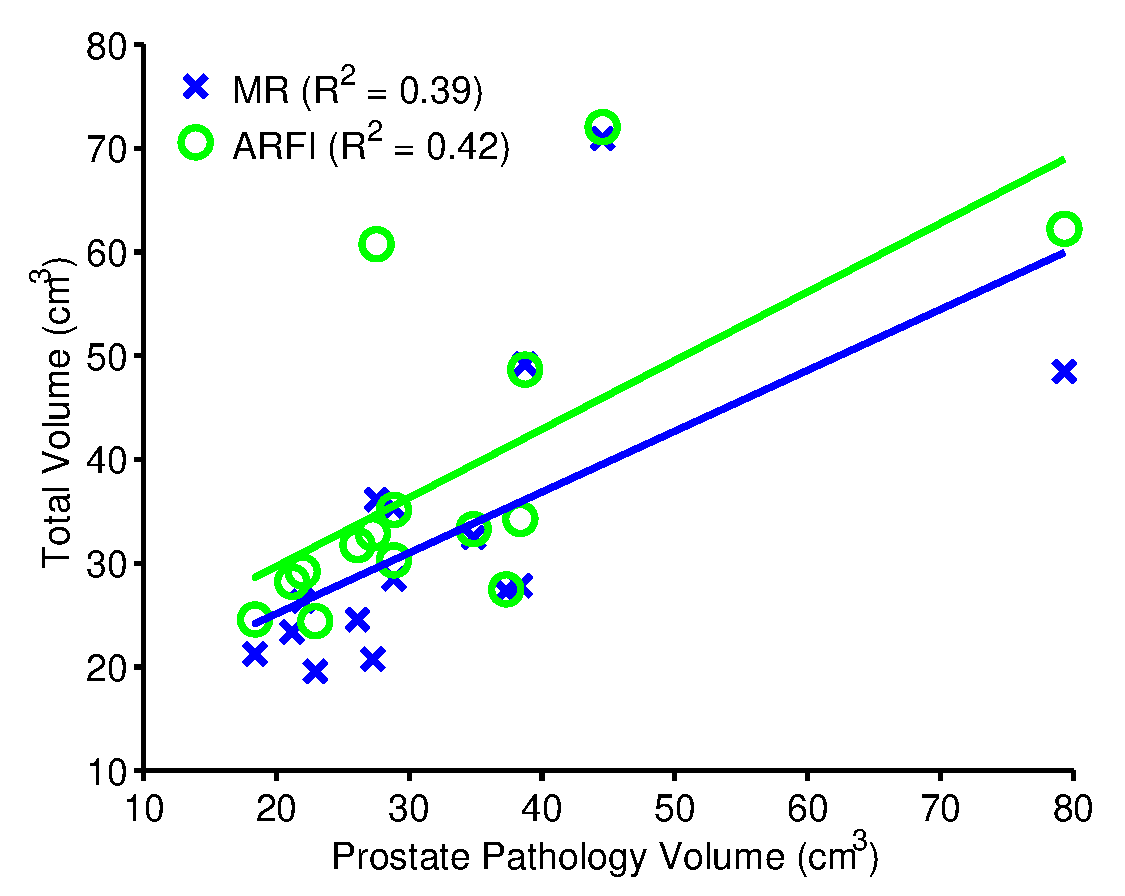
\includegraphics[width=0.3\linewidth]{figs/corr_pathVol_vol_no4} \\
%(d) Image Volume : Prostate Weight (-4) & (e) Image Volume : Path Volume (-4) \\
%\end{tabular}
\caption{Tri-axial pathology measurements were used to make an ellipsoidal
    prostate volume approximation based on gross pathology axis measurements,
    which was moderately well-correlated with the excised prostate weights (a,
    R$^2$ = \pathVolWeightRsq).  T2WI MR (blue, X) showed a moderate
    correlation between the reconstructed volumes and prostate weight (R$^2$ =
    \weightMRrsq), while volumes reconstructed from ARFI images (green, O)
    showed weaker correlation (R$^2$ = \weightARFIrsq) (b).  Weaker
    correlations existed between both T2WI MR and ARFI image volumes and
    approximated ellipsoidal prostate pathology volumes (R$^2$ =
    \pathVolMRrsq~and \pathVolARFIrsq, respectively) (c).  There was one
    pathology specimen that had an erroneous prostate volume and weight
    recorded, which has been excluded from the linear regressions (magenta
    circles).}
\label{fig:mr_arfi_weight}
\end{figure}
